\section{Recursion and language infinity}

Recursive grammars play a crucial role in generating infinite languages.
\begin{definition}[\textit{Recursive derivation}]
    A derivation $A\overset{n}{\implies}xAy$ is considered recursive if $n \geq 1$. 
\end{definition}
\begin{definition}[\textit{Immediately recursive derivation}]
    When $n=1$, the derivation $A\overset{n}{\implies}xAy$ is termed immediately recursive.
\end{definition}
\begin{definition}[\textit{Recursive nonterminal}]
    In the derivation $A\overset{n}{\implies}xAy$, the symbol $A$ is referred to as a recursive nonterminal. 
\end{definition}
\begin{definition}[\textit{Left recursive derivation}]
    If $x=\varepsilon$, the derivation $A\overset{n}{\implies}xAy$ is labeled as left recursive.
\end{definition}
\begin{definition}[\textit{Right recursive derivation}]
    When $y=\varepsilon$, the derivation $A\overset{n}{\implies}xAy$ is denoted as right recursive.
\end{definition}
It is important to emphasize that a grammar can possess recursion without exhibiting circularity.

\paragraph*{Language infinity}
The condition both necessary and sufficient for the language $L(G)$ to be infinite is that, assuming the grammar $G$ is clean and devoid of circular derivations, it permits recursive derivations.
\begin{proof}
    We prove the necessary condition.
    If no recursive derivation is possible, every derivation would have a finite length, implying that $L(G)$ would be finite.
\end{proof}
\begin{proof}
    We prove the sufficient condition.
    The derivation $A\overset{n}{\implies}xAy$ implies the derivation $A\overset{+}{\implies}x^mAy^m$ for any $m \geq 1$ with $x,y \in \Sigma^\ast$ not both empty. 
    Additionally, the cleanliness of $G$ implies that $S\overset{\ast}{\implies}uAv$, indicating that $A$ is reachable from $S$. 
    It also implies that $A\overset{+}{\implies}w$, signifying that the derivation from $A$ terminates successfully. 
    Therefore, nonterminals exist that generate an infinite language.
\end{proof}
\begin{property}
    A grammar lacks recursive derivations if and only if the graph of the produce relation is acyclic.
\end{property}
\begin{example}
    Consider the following grammar:
    \[\begin{cases}
        S \rightarrow aBc \\
        B \rightarrow ab \mid Ca \\
        C \rightarrow c
    \end{cases}\]
    The corresponding graph of the produce relation is depicted below:
    \begin{figure}[H]
        \centering
        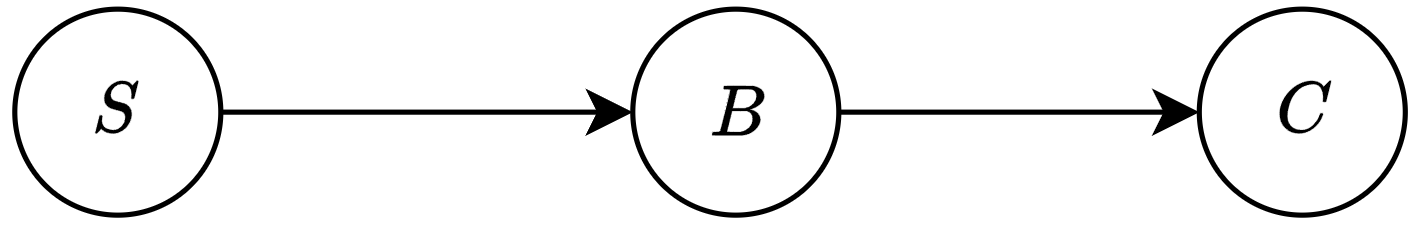
\includegraphics[width=0.5\linewidth]{images/produce.png}
    \end{figure}
    This acyclic graph indicates that the grammar is non-recursive.
\end{example}